

\begin{Schunk}
\begin{Soutput}
## RStudioGD 
##         2
\end{Soutput}

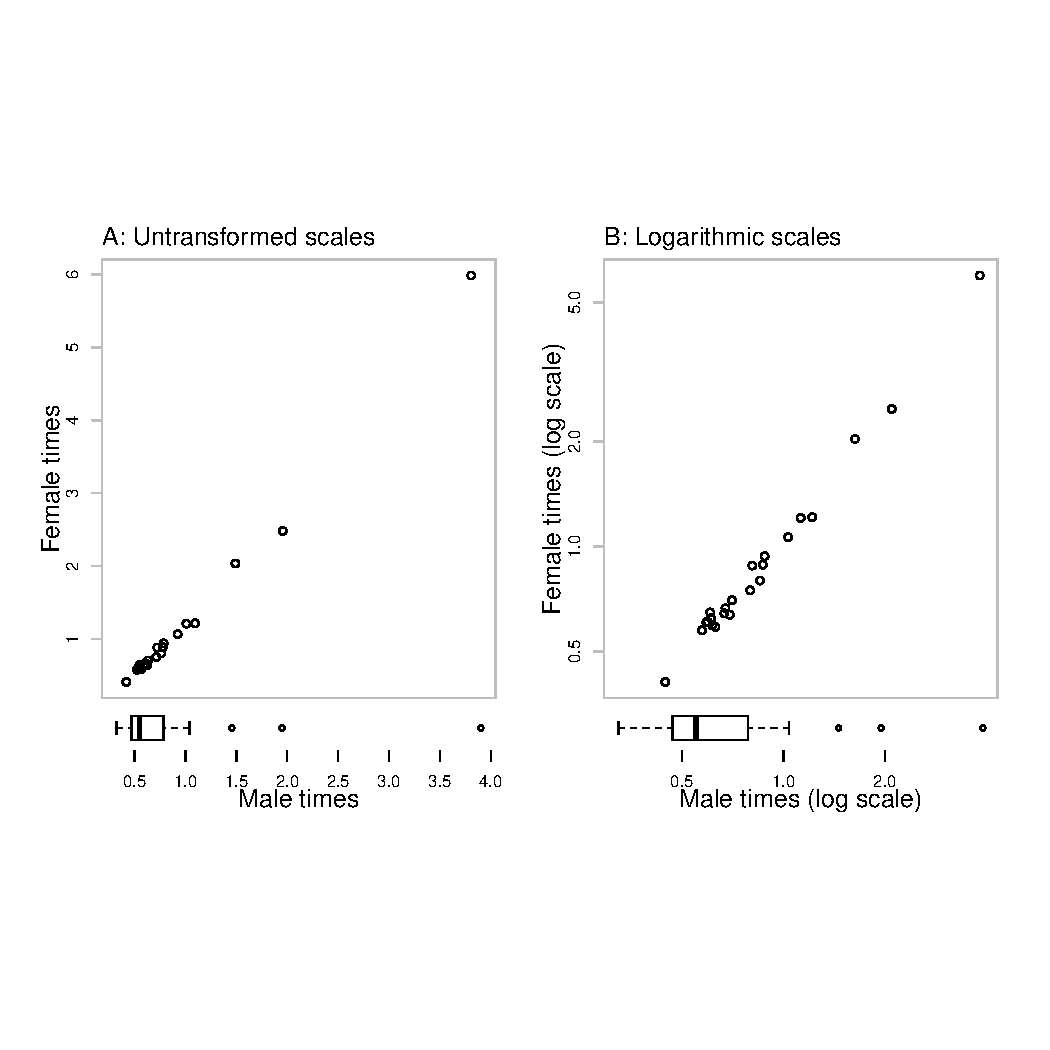
\includegraphics[width=\maxwidth]{figure/unnamed-chunk-2-1} \end{Schunk}

This chapter will describe a range of abilities that create displays
which the user can then manipulate dynamically.  Note in particular
the {\em rgl} and {\em googleVis} packages, designed for interactive
exploration of dynamic changes in relationships with time.  It
reproduces most of the abilities of Google's Public Data Explorer,
which can be accessed at \url{http://www.google.com/publicdata/home}

\section{Dynamic Graphics -- \textit{rgl}}\label{sec:dynamicg}



\begin{figure}
\begin{Schunk}


\centerline{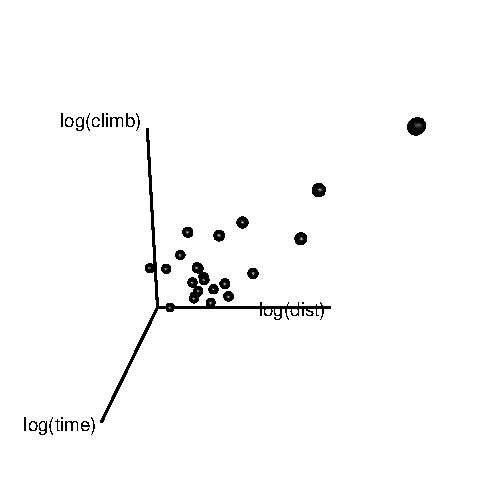
\includegraphics[width=0.625\textwidth]{figs/10-rgl-demo-1} }

\end{Schunk}
\caption{Snapshot of a 3-D dynamic display, for the \txtt{nihills}
data from the {\em DAAG} package.  The display has been dragged to a
position where points very nearly fall on a line.}\label{fig:rgl-ex}
\end{figure}

The \textit{rgl} package provides three-dimensional dynamic graphics.
Use of the functions \txtt{scatter3d()} and \txtt{identify3d()} from
the \emph{car} package may be more convenient for novices than the
\emph{rgl} functions that they call.
Figure \ref{fig:rgl-ex} shows a snapshot of the plot obtained for the
\txtt{nihills} data from the {\em DAAG} package.

\noindent
The following loads the needed packages:
\begin{Schunk}
\begin{Sinput}
## The car and rgl packages must be installed
library(rgl, quietly=TRUE)
library(car, quietly=TRUE)
rgl::setupKnitr()
knit_hooks$set(rgl=hook_rgl)
\end{Sinput}
\end{Schunk}

Code for the figure is:
\begin{Schunk}
\begin{Sinput}
library(DAAG, quietly=TRUE)
open3d()            # Precedes the call to par3d()
par3d(cex=0.75)     # Optional
                    # Other params: see help(par3d)
with(nihills, scatter3d(x=log(dist), y=log(climb),
                        z=log(time),
                        grid=FALSE,
                        surface=FALSE,
                        point.col="black",
                        axis.scales=FALSE))
## NB: Use middle or right mouse button to drag a
## rectangle around a point that is to be labeled.
\end{Sinput}
\end{Schunk}
\marginnote[11pt]{Use \txtt{rgl.snapshot()} to save the current plot
  into a file.}

Use the function \txtt{identify3d()} to start the identification of
points.  Following the call to \txtt{identify3d()}, use the middle (or
maybe right) mouse button to drag a rectangle around any point that is
to be labeled.  To cease identifying points, make a middle (or right)
click on an empty region of the plot.  The labels may appear only at
this point.  Here, for identification of points shown in Figure
\ref{fig:rgl-ex}, is suitable code:
\begin{Schunk}
\begin{Sinput}
with(nihills, identify3d(x=log(dist), y=log(climb),
                         z=log(time),
                         labels=row.names(nihills),
                         col="gray"))
\end{Sinput}
\end{Schunk}

Such a plot can be helpful in identifying high leverage points,
e.g., in the regression of \txtt{log(time)} on \txtt{log(dist)}
and \txtt{log(climb)}.  The plot needs to be rotated to give a view
in which the leverage is apparent.

\subsection*{The  \texttt{rggobi} package}

The \textit{rggobi} package offers a wider range of features, via an
interface to the GGobi system.  For installation details go to
\url{http://www.ggobi.org/}.  Windows users can use the following to
install all the required files from an R session that has access to a
live internet connection:
\begin{Schunk}
\begin{Sinput}
source("http://www.ggobi.org/downloads/install.r")
\end{Sinput}
\end{Schunk}

\section{The {\em googleVis} Package}\label{sec:gvis}

This provides an interface to the abilities of Google's Public Data
Explorer.  While these abilities can be accessed from the web page
noted below, there are obvious advantages in setting up the display
from one's own computer.\sidenote{An internet connection is needed to
  access Google's API (Application Program Interface) when the chart
  is displayed.}

\subsection{Google's Public Data Explorer}

Upon accessing Google's web page
\url{http://www.google.com/publicdata/home}, the display will cycle
through examples of the use of Motion Charts, and other related
charts.  Click on \underline{Explore Data} to go to the interactive
version of the relevant display.\sidenote{Various controls are placed
  in the margins of the graph.  Move the pointer over one or other
  control feature to get information on its purpose, or over a point
  to display information about that point. For changing the $x$-
  and/or $y$- variables, or for changing the variable that determines
  point size, click on the relevant downward pointing selector arrow.
  Scales, separately for the two axes, can be either linear or
  logarithmic.}  These charts, which are interesting in themselves,
show the abilities that {\em googleVis} is designed to emulate.  See
the annotations in Figure \ref{col:mchart} below for details that
should be enough to get started.

A slider below the graph can be moved to show how the relationships
that are plotted change over the available timespan, commonly 1960
through to 2010 (but note that not all data will be available for all
years).  Click on the solid right-pointing triangle on the left of
the slider scale to see the graph changing dynamically in moving from the
currently shown year through to 2010.

\subsection{Use of {\em googleVis} to create motion charts}\label{ss:gvis}

\begin{SaveVerbatim}{gvis}
vignette("googleVis")
\end{SaveVerbatim}

The details given here should be supplemented with examination
of the vignette\marginnote{To display the vignette, type:
\vspace*{-7pt}

\UseVerbatim[fontsize=\relsize{0}]{gvis} } that accompanies the {\em
googleVis} package.  Note especially Figure 1 on page 5 of the
vignette.

Creation of a motion chart, once the data is in place, is remarkably
straightforward. The starting point is a data frame in that has a
column (e.g.\ Countries) that can be used as an \txtt{id} variable, a
column (e.g.\ Year) that has a \txtt{timevar} variable, and columns
that can be used to supply $x$- and $y$- variables.  Optionally,
columns may be identified for use as a \txtt{colorvar} and/or a
\txtt{sizevar}.

The dataset \txtt{grog} from the {\em DAAG} package has a suitable
structure.  One can create a motion chart thus:
\begin{minipage}[t]{1.075\textwidth}
\begin{Schunk}
\begin{Sinput}
library(googleVis)
M <- gvisMotionChart(grog, id="Country", timevar="Year")
## This next line requires a live internet connection,
## and Adobe Flash must be installed.
plot(M)
\end{Sinput}
\end{Schunk}
\end{minipage}
If the browser window that appears displays 'Flash' in gray in the
middle of the screen, click there to proceed.  A browser window with a
gray display region should appear.

For the \txtt{grog} dataset, the Motion Chart does a less satisfactory
job than Figure \ref{fig:allgrog} in Section \ref{ss:grog}.  Motion
charts come into their own for the examination of steady changes over
time in a bivariate relationship, with different patterns of
relationship for different subgroups of the data.

A plot that allows the display of various World Bank development
indicators can be obtained by typing:\marginnote{The code used to
  download the data and display the motion chart will appear on your
  screen.}
\begin{Schunk}
\begin{Sinput}
demo(WorldBank)
\end{Sinput}
\end{Schunk}
This can take a while to start up -- data has to be downloaded from
the World Bank web site. Hover the mouse pointer over features that
appear in the margins of the display to see annotation that indicates
how you can change or manipulate various aspects of the display.

The data from the World Bank site is stored into a data frame
\txtt{WorldBank}.  The command that creates a gvis object M
is:\sidenote{Both \txtt{WorldBank} and \txtt{M} should be in your
  workspace after running \txtt{demo(WorldBank)}.  The data are
  also alternatively available from the image file
\txtt{WorldBank.RData} at the url noted
on the reverse of the title page.}
\begin{Schunk}
\begin{Sinput}
M <- gvisMotionChart(WorldBank, idvar="country",
          timevar="year",
          xvar="life.expectancy",
          yvar="fertility.rate",
          colorvar="region", sizevar="population",
          options=list(width=700, height=600))
## Now display the motion chart
plot(M)
\end{Sinput}
\end{Schunk}
Change \txtt{width} and \txtt{height} as needed to make better
use of the screen display.

If arguments are supplied, security setting issues on the user
computer can result in an initial assignment of columns that does not
accord with the supplied arguments.\sidenote{The
  {\em gvis} object M comprises Javascript code that can be
  included on a web page.  This should display correctly when the web
  page is accessed.}  The drop-down menus should however function
correctly, and can be used to obtain a display that accords with any
choice of arguments that the user may want.

For a further example, load the image file {\bf wdiSel.RData},
available from the url noted on the reverse of the title page. This
will make available the data frame \txtt{wdiSel}. This has a larger
number of indicators, but for 26 countries only.  Figure
\ref{col:mchart} (with the figures that are shown in color) shows an
annotated version of a motion chart that was created from this
dataset.

The following code generated the initial chart.  The change
to a log scale on the vertical axis was made interactively:
\begin{fullwidth}
\begin{Schunk}
\begin{Sinput}
xnam <- "Electric power consumption (kWh per capita)"
ynam <- "Mobile cellular subscriptions (per 100 people)"
M <- gvisMotionChart(wdiSel, idvar="Country.Name", timevar="Year",
                     xvar=xnam, yvar=ynam,
                     colorvar="region", sizevar="Population, total",
                     options=list(width=600, height=500),
                     chartid="wbMotionChartSel")
plot(M)
\end{Sinput}
\end{Schunk}
\end{fullwidth}
